\chapter{Advances in Soft-Computational Approaches in the Design of Microstrip Antennas and Arrays}
\label{chap:chap2}
\section{Background} \label{c2sec_background}
Antenna design technologies have significantly advanced in the last decade. Computer aided methods are emerging as a solution to build more complex patch antennas and arrays with better efficiency and performance. Soft-computational approaches in the design of antennas and arrays have unleashed highly optimized geometries that cannot be designed by humans. This advancement has contributed towards the development of compact and reliable communication gadgets that are crucial in connecting the whole world.

\subsection{Design of Microstrip Antennas}
Microstrip antennas are low profile, light, conformal and durable antennas which are ideal for use in portable and compact communication devices. Microstrip antennas are usually fabricated on a PCB board which can be integrated with other electronic circuits easily. There are three approaches for the analysis and designing of microstrip antennas:
\begin{itemize}
\item Transmission line model
\item Cavity model
\item Full-wave model
\end{itemize}

The transmission model and the cavity model have been used for analysis and synthesis of microstrip antennas for several decades. The two models are analytical in nature and hence provides high insights into the working of an antenna. The accuracy of these models, however, is not high. Full-wave models, on the other hand, yield very high accuracy. These models numerically solves wave equations with boundary conditions defined by the geometrical structure of an electromagnetic solver. These models yield highly accurate estimation of the behavior of an antenna. These knowledge are not suitable for analytical study of an antenna or explaining the behavior of a structure \cite{balanis}.

For a simple rectangular or circular patch, it is easy to design or study an antenna analytically using either a transmission line model or a cavity model. However, for arbitrarily shaped antennas, it is difficult to formulate a transmission line model or a cavity model. This adds up to the challenges in antenna design. Further, these antennas need fine-tuning in order to achieve desired performance at the frequencies of interest. Due to the inaccuracies of the transmission line model and the cavity model, regularly shaped antennas also needs fine-tuning and optimization. This process is time and labor intensive and requires a significant expertise of the domain.

Because of the limitations of the traditional approaches for antenna design, soft-computational approaches are becoming popular. An evolutionary algorithm can be used to search the design space and automatically find novel antenna designs that are more effective than would otherwise be developed \cite{cadNASA}. Evolutionary-based approaches in antenna design are largely explored in the recent years. Various soft-computational techniques have been used to design antennas of various sizes and shapes. Sometimes, the algorithms are also tailored to make them more suitable for this purpose.

\subsection{Design of Antenna Arrays}
Antenna arrays are very important in the design of directional communication system. Arrays are inevitable in modern-day communication systems which make use of spatial diversity. The far-field radiation pattern of an array can be electrically steered by adjusting the phase of excitation of each individual element of an array. Similarly, it is possible to avoid interference from a specific direction by generating a null along that direction. A MIMO communication system is a good example of arrays in modern-day communication. Arrays with electrically steerable beams are also used in radars.

A thinned array or a sparse array is an array in which the number of elements of the array is reduced in such a way that the performance in terms of the radiation pattern and gain of the array is not significantly compromised. Sparse arrays help in reducing the size and complexity of the RF circuitry required for exciting each element at a different phase. Design of sparse array is another field in which soft-computational approaches are becoming popular.

Other problem in the array design includes side-lobe level (SLL) reduction and impedance matching. In SLL reduction, the primary objective is to reduce the power of the antenna along the side lobes and maximize the gain of the antenna along the main lobe in the desired direction. The objective of an impedance matching problem in array design is to make sure that the input impedance of each of the elements in an array is properly matched with that of the respective feeding lines. Soft-computational approaches are explored in both of these cases.

\section{Problems in Soft-Computational Approaches for Antenna and Array Design} \label{c2sec_problems}
The common design problems in microstrip antennas include reduction of the electrical size of the antenna, enhancement of gain, enhancement of bandwidth, obtaining desired polarization performance, the design of filter integrated with antennas etc. In this section, some of the popular problems of evolutionary-based approaches in the design of microstrip antennas and arrays are discussed.
\subsection{Antenna Design Problems}
Optimization problems in antenna design can be broadly classified into two categories --
\begin{itemize}
\item Continuous problem
\item Binary problems
\end{itemize}

Optimizing various dimensions of an antenna is an example of a continuous problem. In a binary problem, the primary objective is usually to find the presence (0) or absence (1) of metal in a position to find the shape of the patch.

In \cite{patch_miniaturize_ga}, the dimensions of a rectangular patch antenna are optimized using genetic algorithm (GA). Five physical dimensions of the antenna are tuned algorithmically to optimize the antenna as shown in Figure \ref{fig_2_1}. This is a 5-dimensional continuous problem. Here, the antenna is simulated in CST studio in order to calculate the cost function and the genetic algorithm is implemented in MATLAB.

\begin{figure}
  \centering
  \includegraphics[width=0.3\linewidth]{fig_2_1.eps}\\
  \caption[Frequency reconfigurable E-shaped patch design schematic using RF switches with optimization parameters listed.] {Frequency reconfigurable E-shaped patch design schematic using RF switches with optimization parameters listed. \cite{patch_miniaturize_ga}} \label{fig_2_1}
\end{figure}

\begin{figure}
  \centering
  \subfigure[Divisions of the rectangular patch]{
\includegraphics[width=0.3\linewidth]{fig_2_2a.eps}}~~~~~~~~~~~~~~~~~~~~~
  \subfigure[Optimized antenna]{\includegraphics[width=0.3\linewidth]{fig_2_2b.eps}}\\
  \caption [Division of the patch (Dark: metal, White: without metal) (a) Division of patch area (b) optimized patch]{Division of the patch (Gray: metal, White: without metal) (a) Division of patch area (b) optimized patch \cite{optPatch}} \label{fig_2_2}
\end{figure}

An example of a discrete problem is \cite{optPatch}. In this work, binary particle swarm optimization (PSO) technique is used to design a wide-band antenna. In this work, initially, a rectangular patch is taken. The patch is divided into smaller blocks in which the presence and absence of metallization are found using the binary PSO. The original rectangular patch antenna and the final design are shown in Figure \ref{fig_2_2} (a) and (b) respectively. The optimized antenna is basically a slotted rectangular patch antenna in which the position of the slots is obtained algorithmically. The final design has an irregular geometry. The frequency responses of the return loss ($S_{11}$) parameter of the antenna before and after optimization are shown in Figure \ref{fig_2_3}.

\begin{figure}
  \centering
  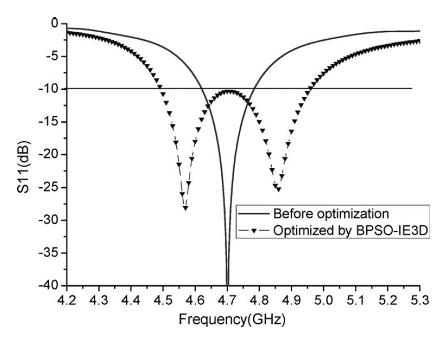
\includegraphics[width=0.6\linewidth]{fig_2_3.eps}\\
  \caption [Computed $S_{11}$ curves versus frequency]{Computed $S_{11}$ curves versus frequency. \cite{patch_miniaturize_ga}} \label{fig_2_3}
\end{figure}

In \cite{freqReconfCogn} a similar approach is presented using GA for designing an antenna for cognitive radio application. In this work, the optimization is applied to find the slot shape and the switch locations in the ground plane of monopole antennas for adjustment of the bandwidth. Here, the switches in the ground plane help in exciting the antenna at different modes. Each mode has its own resonant frequency. Hence, using the switch the resonant frequency of the antenna can be tuned. With an optimum number of switches, the frequency tuning can be performed by adjusting the minimum possible number of switches without compromising the performance of the antenna.

\subsection{Array Synthesis Problems}
The three crucial conditions for a linear array to meet are \cite{arraySynth1}:
\begin{itemize}
\item \textbf{Gain maximization in the desired direction:} Gain maximization refers to maximizing the far field gain of the antenna along the desired direction in the polar coordinate system defined by azimuth angle ($\phi$), and elevation angle ($\theta$).
\item \textbf{Side-lobe level (SLL) reduction:} SLL reduction refers to suppression of the gain of the antenna array in all directions except the direction of the maximum gain.
\item \textbf{Impedance matching:} In an array, each element is excited individually by a microstrip line in the feeding network. The feed line usually follows a phase shifter or a switch. The objective of the impedance matching problem in array synthesis is to make sure that the complex impedance of each element of the array is matched with the corresponding feed line for each operating mode of the array. If the impedances are not properly matched in an array, the radiation efficiency will be poor.
\end{itemize}

In \cite{arraySynth1}, Z. D. Zaharis et al. proposed a soft-computational approach to design an array that meets all these conditions. In this work, Boolean Particle Swarm Optimization (PSO) technique is used. A large number of evolutionary approaches have been explored worldwide by researchers to design arrays with significant SLL reduction. In \cite{arraySynth2}, the side lobe level of a time modulated linear array is suppressed using non-dominated sorting genetic algorithm II (NSGA-II). Here, the array factor (AF) of the linear array is mathematically represented in terms of Fourier series. The static excitation and the ``switch on'' time are optimized using the NSGA-II algorithm to minimize the SLL of the array. In \cite{arraySynth3} a new optimization algorithm known as Teaching Learning Based Optimization (TLBO) is applied for SLL reduction. Here also, the excitation parameters are optimized for a linear array to reduce SLL. SLL reduction problem is addressed for both linear as well as circular arrays in \cite{arraySynth4} using a hybrid optimization technique called cuckoo search-chicken swarm optimization (CSCSO). CSCSO combines cuckoo search (CS) which is a global search algorithm and chicken swarm optimization (CSO) which introduce a hierarchy mechanism.

In \cite{compCAD4Arry}, the authors have compared GA, PSO, and DE for the design of a scannable circular array. The designed circular array has a full 360 degree scan at steps of 30 degree. In this work also, optimization techniques are used to calculate the excitation parameters of each element of the array so that gain is maximized along a given direction and SLL is minimized. It is observed from the experimental results presented in \cite{compCAD4Arry} that all the three algorithms yield better performance compared to the conventional case in terms of gain maximization and SLL reduction. However, the results from the different methods are not the same; this is mainly because the algorithms do not guarantee convergence to the global optimum in finite time.

\subsection{Array Thinning Problems}
Thinning of antenna arrays involves the removal (turning off) of some elements in the antenna array so as to maintain radiation properties similar to that of the fully populated array, but using a lower number of elements. In a thinned array, the spacing between the elements is not uniform. Thinning a large array helps in further reducing its SLL and also reducing the number of antennas in the array and thereby substantially cutting down the cost. In most of the cases, analytical approaches are not cost-effective for array thinning problems and therefore soft-computational approaches are most widely used.

In \cite{arrayThin1}, a thinned concentric planar circular antenna array of isotropic elements is designed to generate a pencil beam in the vertical plane with reduced side lobe level and increasing number of switched off elements using an improved variant of DE, called Differential Evolution with Global and Local neighborhoods (DEGL). Another new optimization algorithm called the binary spider monkey optimization (SMO) algorithm for designing a thinned concentric circular array is proposed in \cite{arrayThin2}. The array thinning of a concentric circular antenna array is illustrated in Figure \ref{fig_2_4}.

\begin{figure}
  \centering
  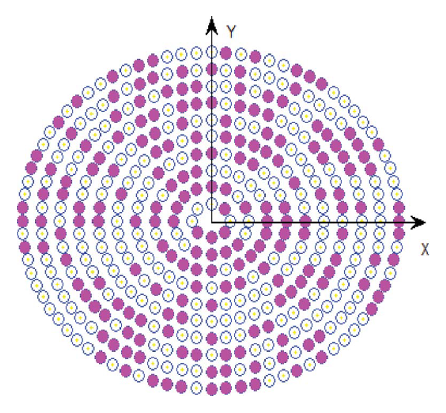
\includegraphics[width=0.35\linewidth]{fig_2_4.eps}\\
  \caption [Isotropic elements (dark shows ON and light as OFF) in ten ring concentric circular antenna array]{440 isotropic elements (dark shows ON and light as OFF) in ten ring concentric circular antenna array. \cite{arrayThin2}} \label{fig_2_4}
\end{figure}

Binary butterfly mating optimization (BBMO) algorithm along with a subarray strategy for thinning of antenna array is proposed in \cite{arrayThin3}. Here, the subarray strategy divides the linear array into two parts, one part with a fixed number of element turned on in the middle of the array and the rest elements on the edge of array composing another subarray. In order to reduce the complexity of the thinning process, BBMO algorithm is used to optimize the element on the edge of an array. The proposed BBMO with subarray strategy is used to synthesize a linear sparse antenna array in order to reduce maximum sidelobe level and at the same time keeping the percentage of thinning equal to or more than the desired level.

\subsection{Evolutionary Design of Metamaterial Structures}
Electromagnetic metamaterials are engineered materials that can yield a negative value of its permittivity ($\epsilon$) or permeability ($\mu$) or both at a frequency band of interest. Traditional metamaterial structures include the split ring resonator (SRR), the complementary split ring resonator (CSRR), electromagnetic band-gap (EBG) structures etc. These structures are either built periodically within a dielectric block or fabricated on the surface of an electromagnetic device. A wide range of research works has reported enhancement of the performance of microstrip antennas, wave-guides and other microwave devices on the use of metamaterial structures.

One of the earliest works that reported the use of evolutionary-based approaches in the design of a metamaterial unit cell is \cite{optMtm}. Here, genetic algorithm is used to design a metametarial unit cell with negative value of $\mu$ using the filling element methodology. Here square and hexagonal pixels are considered for the design of the metamaterial unit cell. The evolution of the metamaterial structure in this case is illustrated in Figure \ref{fig_2_5}. A similar work for design of metamaterial unit cell using topology optimization is reported in \cite{lh_mtm}.

\begin{figure}
  \centering
  \includegraphics[width=0.35\linewidth]{fig_2_5.eps}\\
  \caption[The best fitness plotted as a function of generation (top). The unit cells show the best structures (elite) at different generations during the evolution process of the GA (bottom)]{The best fitness plotted as a function of generation (top). The unit cells show the best structures (elite) at different generations during the evolution process of the GA (bottom). \cite{optMtm}} \label{fig_2_5}
\end{figure}

\subsection{Evolutionary Design of Metasurfaces}
Metasurfaces are controllable smart surfaces that have a wide range of applications in the design of antennas and other electromagnetic devices. Metasurfaces were proposed in \cite{metasurface1} as a two-dimensional equivalent of the three-dimensional resonant particle type metamaterials. Later, single metamaterial unit cells, also known as planar metamaterials became popular. In the recent years, planar metamaterial unit cells (such as SRR, CSRR, Mushroom-Type EBG unit cell etc.) have been widely reported in the design of microstrip antennas, filters, phase-shifters etc. However, metasurfaces are nowadays incorporated with arrays to reduce the mutual coupling between elements \cite{metasurface2}. In a metasurface based design of microstrip antenna array, the array is sandwitched between two dielectric substrates. The lower face of the lower substrate has the ground plane and the upper face of the upper substrate has the metasurface. The structure is illustrated in Figure \ref{fig_2_6}.

\begin{figure}
  \centering
  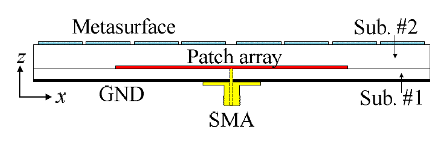
\includegraphics[width=0.6\linewidth]{fig_2_6.eps}\\
  \caption [Cross sectional view of a meta-surface based microstrip antenna array]{Cross sectional view of a meta-surface based microstrip antenna array \cite{metasurface2}} \label{fig_2_6}
\end{figure}

Design of metasurfaces is one of the highly emerging techniques for the improvement of antenna arrays. Genetic algorithm is used for optimization purposes in the design of programmable metasurfaces for active dynamic polarization, scattering and focusing control in \cite{softCompMeta}. In a similar work \cite{uwb_rcs}, a metasurface is designed for reduction of radar cross section (RCS) of an antenna array using polarization convertor and genetic algorithm.

\section{Techniques and Methods for the use of Soft-Computational Approaches in Design of Antennas and Arrays} \label{c2sec_methods}
So far, the various problems in the use of soft-computational approaches for the design of microstrip antennas, arrays and metamaterials are discussed. In this section, the various methods and techniques for the use of soft-computational approaches in the design of antennas and other electromagnetic devices are discussed briefly.

\subsection{Evolutionary Optimization Algorithms}
Evolutionary optimization algorithms are inspired by nature. One of the most commonly used evolutionary algorithm is the genetic algorithm (GA). It mimics the Darwin's theory of natural selection in the evolution of a species. Particle swarm optimization (PSO), another popular algorithm mimics swarm intelligence that include the behavior of ant colonies, bird flocking, animal herding, bacterial growth, fish schooling and microbial intelligence. Differential evolution (DE) is another popular algorithm that is widely used in antenna design. None of these algorithms guarantee global maxima, and based on problem the performance of the algorithms vary \cite{compCAD4Arry}.

In the design of antennas, metamaterial structures and arrays, most of the optimization problems are discrete value problems. The classical GA, PSO, and DE are, on the other hand, designed for continuous value problems. However, there are several variants of these algorithms to address discrete value problems. These methods include binary-coded genetic algorithm (BGA) \cite{optAlgBGAbook, optAlgEMbook}, Binary PSO (BinPSO) \cite{optAlgBPSO}, Boolean PSO \cite{arraySynth1, OptAlgBoolPSO4Ant}, Binary differential evolution \cite{optAlgBinDE, optAlgModBinDE}. In \cite{optAlgDE4AntennaRev}, a detailed analysis of these algorithms is presented along with design of a patch antenna and an array using the novel binary differential evolution (NBDE) algorithm presented in \cite{optAlgModBinDE}.

Apart from these standard evolutionary algorithms, many new evolutionary algorithms have been presented in the recent years. Some of these algorithms, enlisted as follows, are reported in the design of antennas and array design.

\begin{itemize}
\item Teaching learning based optimization (TLBO) algorithm \cite{arraySynth3}
\item Chicken swarm optimization (CSO) algorithm \cite{arraySynth4}
\item Spider monkey optimization (SMO) algorithm \cite{arrayThin1}
\item Binary butterfly mating optimization (BBMO) algorithm \cite{arrayThin2}
\item Cuckoo search (CS) algorithm \cite{CuckooSerach}
\item Invasive Weed Optimization (IWO) \cite{InvasiveWeed}
\end{itemize}

\subsection{Method for Array Synthesis Problems for SLL Reduction and Gain Maximization} \label{c2subsec_sll_methods}
An array comprises of identical antenna elements of known radiation pattern. It is therefore possible to analytically derive the cost function of the optimization problems as in \cite{arraySynth2, arraySynth3, arraySynth4, compCAD4Arry}. The optimization algorithm is used to determine the excitation parameters of each of the elements of the array in order to meet the desired goal of gain maximization or SLL reduction.

In an array, each element is excited separately. In a broad-side array where the main lobe is along a direction perpendicular to the array axis, each element is excited at same phase. In this case, the magnitudes of the excitation parameters are optimized to maximize the gain of the antenna and minimize the SLL. In a scannable array each antenna element is excited at different variable phase. The phase angles are adjusted to tune the direction of the main lobe. In this case, the array factor corresponding to every possible scanning step is optimized by adjusting the magnitudes as well as phase angles of excitation of each antenna element in the array. A computational tool such as MATLAB is sufficient for solving such problems.

When an array synthesis problem includes impedance matching, a full wave model or a surrogate model is required to be incorporated in the system which adds up to the complexity of the problem. These two approaches are discussed in the following sections \ref{c2subsec_thinning} and \ref{c2subsec_tools} respectively.

\subsection{Method for Array Thinning Problems} \label{c2subsec_thinning}
An array thinning problem is initialized with a fully populated array. A binary optimization algorithm is then used to turn off certain elements of the array so that the effect on the overall radiation pattern of the array is insignificant. In such problems also the elements are identical with known far-field radiation patterns. Hence, the cost function of the problem can be derived analytically.

In \cite{arrayThin1, arrayThin2, arrayThin3}, arrays of isotropic antenna elements are used. MATLAB is used in \cite{arrayThin2} and \cite{arrayThin3}. In all these works, the cost function is in terms of SLL reduction. When some elements of a large array are turned off, the SLL of the array increases. Hence, SLL plays a significant role in an array thinning problem. The SLL can be obtained from analytically derived mathematical expressions or from a full wave solver.

\subsection{Interface between Computational Tool and EM Solver} \label{c2subsec_tools}
In order to evaluate the performance of an antenna or an array with high accuracy, a full wave EM solver such as HFSS, CST Studio, IE3D etc. is essential. Optimization algorithms, on the other hand, needs specialized computational tools such as MATLAB. In an evolutionary approach, each generation of the antenna requires independent analysis in order to compute the cost function. In the methods discussed in above Sections \ref{c2subsec_sll_methods} and \ref{c2subsec_thinning}, the cost function is calculated from analytically derived expressions. However, for design of a single antenna element \cite{patch_miniaturize_ga, optPatch, freqReconfCogn} or an array synthesis problem involving impedance matching \cite{arraySynth1}, such an approach is not reliable. It is therefore necessary to integrate the computational tool and the EM solver, so that the antenna is iteratively designed and evaluated with high accuracy.

The flow diagram of genetic algorithm based design of a rectangular patch antenna reported in \cite{patch_miniaturize_ga} is shown in Figure \ref{fig_2_7}. It is observed from the figure that the antenna is modeled in CST studio, which is a full-wave EM solver. The genetic algorithm is implemented in MATLAB. Such arrangement helps in accurate evaluation of the antenna for the best performance.

\begin{figure}
  \centering
  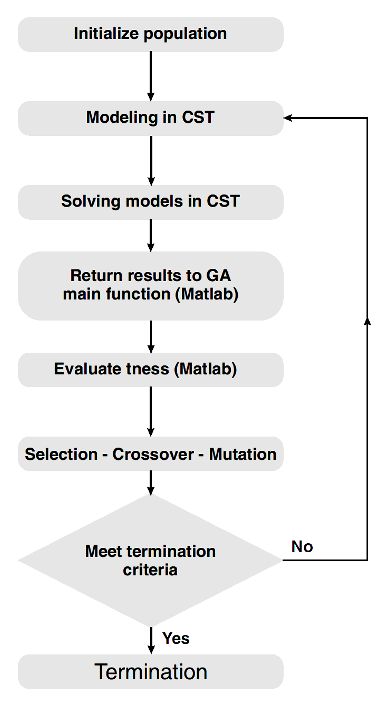
\includegraphics[width=0.4\linewidth]{fig_2_7.eps}\\
  \caption[A block diagram of genetic algorithm function used in this design]{A block diagram of genetic algorithm function used in this design \cite{patch_miniaturize_ga}} \label{fig_2_7}
\end{figure}

In \cite{optPatch}, the EM solver used is IE3D. Here, the design parameters are written to a file which is read by the IE3D solver. After simulation, the IE3D solver writes the data to another file which is read from MATLAB for computation of the cost function and the design parameters for the next iteration. A custom EM solver is used in \cite{arraySynth1} for an array synthesis problem involving impedance matching in a similar approach.

HFSS, another popular EM solver tool, supports a script interface. Any antenna can be designed and analyzed by writing a script. This script interface can be used for the designing of an antenna in MATLAB and exporting it to HFSS. In the script, HFSS may be instructed to store the result in a specified file which can later be read from MATLAB to obtain the simulation results.

\subsection{Surrogate Model Assisted Optimization}
A full-wave EM simulation involves a huge set of computations and hence such simulations are often time consuming. This significantly limits the efficiency of evolutionary approaches for the design of antennas. A solution to this problem is the introduction of a surrogate model. In \cite{antSurrD01}, a surrogate model assisted evolutionary algorithm (SAEA) is proposed. Here, a surrogate model is a Gaussian process model of the actual full-wave simulations. Surrogate modeling methods include Gaussian process or Kriging, response surface methods, artificial neural networks (ANN), support vector machines and radial basis function models. A surrogate model is derived from actual full-wave simulation. At every iteration of the evolutionary algorithm, the cost function is evaluated from the surrogate model instead of the actual full-wave simulation. This significantly enhances the efficiency of the optimization process.

Surrogate models based approaches are being explored for various antenna design problems in the recent years. In \cite{surrMTM01}, a surrogate model assisted optimization technique for metamaterial devices is proposed. Surrogate models are explored in \cite{antSurrConstMO} for constrained, multi-objective antenna design problems.

\section{Conclusion}\label{c2sec_cncl}
The various problems in soft-computational approaches for designing of antennas and arrays are summarized. Soft-computational approaches have a number of advantages over the traditional approaches for antenna design. Evolutionary-based algorithms are basically search algorithms which can find an optimized solution in the solution space. Soft-computational tools can be helpful if the search space is large. Techniques such as surrogate model helps in reducing computation time; however, synthesis of the surrogate model is another area of research.
